%% Icone simple d'un circuit RC (filtre passe-bas), sans reference a
%% l'equation differentielle : entree v_e(t), sortie v_s(t) aux bornes
%% du condensateur. Consomme par slides.
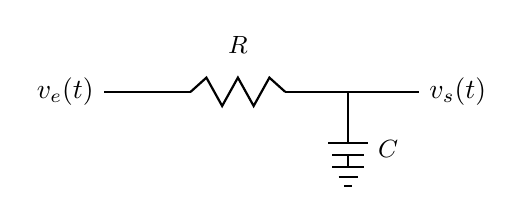
\begin{tikzpicture}[x=1cm,y=1cm, thick]
    % fil d'entree
    \draw (-1.7,1) -- (-0.6,1);
    \node[left] at (-1.7,1) {$v_e(t)$};
    % resistance (zigzag)
    \draw (-0.6,1) -- (-0.4,1.18) -- (-0.2,0.82) -- (0,1.18) -- (0.2,0.82) -- (0.4,1.18) -- (0.6,1);
    \node[above] at (0,1.35) {\small $R$};
    % noeud de sortie
    \draw (0.6,1) -- (1.4,1);
    \draw (1.4,1) -- (2.3,1);
    \node[right] at (2.3,1) {$v_s(t)$};
    % condensateur
    \draw (1.4,1) -- (1.4,0.35);
    \draw (1.15,0.35) -- (1.65,0.35);
    \draw (1.2,0.2) -- (1.6,0.2);
    \node[right] at (1.65,0.28) {\small $C$};
    % masse
    \draw (1.4,0.2) -- (1.4,0.05);
    \draw (1.2,0.05) -- (1.6,0.05);
    \draw (1.28,-0.08) -- (1.52,-0.08);
    \draw (1.35,-0.2) -- (1.45,-0.2);
\end{tikzpicture}
